\documentclass[twoside]{book}

% Packages required by doxygen
\usepackage{fixltx2e}
\usepackage{calc}
\usepackage{doxygen}
\usepackage[export]{adjustbox} % also loads graphicx
\usepackage{graphicx}
\usepackage[utf8]{inputenc}
\usepackage{makeidx}
\usepackage{multicol}
\usepackage{multirow}
\PassOptionsToPackage{warn}{textcomp}
\usepackage{textcomp}
\usepackage[nointegrals]{wasysym}
\usepackage[table]{xcolor}

% Font selection
\usepackage[T1]{fontenc}
\usepackage[scaled=.90]{helvet}
\usepackage{courier}
\usepackage{amssymb}
\usepackage{sectsty}
\renewcommand{\familydefault}{\sfdefault}
\allsectionsfont{%
  \fontseries{bc}\selectfont%
  \color{darkgray}%
}
\renewcommand{\DoxyLabelFont}{%
  \fontseries{bc}\selectfont%
  \color{darkgray}%
}
\newcommand{\+}{\discretionary{\mbox{\scriptsize$\hookleftarrow$}}{}{}}

% Page & text layout
\usepackage{geometry}
\geometry{%
  a4paper,%
  top=2.5cm,%
  bottom=2.5cm,%
  left=2.5cm,%
  right=2.5cm%
}
\tolerance=750
\hfuzz=15pt
\hbadness=750
\setlength{\emergencystretch}{15pt}
\setlength{\parindent}{0cm}
\setlength{\parskip}{3ex plus 2ex minus 2ex}
\makeatletter
\renewcommand{\paragraph}{%
  \@startsection{paragraph}{4}{0ex}{-1.0ex}{1.0ex}{%
    \normalfont\normalsize\bfseries\SS@parafont%
  }%
}
\renewcommand{\subparagraph}{%
  \@startsection{subparagraph}{5}{0ex}{-1.0ex}{1.0ex}{%
    \normalfont\normalsize\bfseries\SS@subparafont%
  }%
}
\makeatother

% Headers & footers
\usepackage{fancyhdr}
\pagestyle{fancyplain}
\fancyhead[LE]{\fancyplain{}{\bfseries\thepage}}
\fancyhead[CE]{\fancyplain{}{}}
\fancyhead[RE]{\fancyplain{}{\bfseries\leftmark}}
\fancyhead[LO]{\fancyplain{}{\bfseries\rightmark}}
\fancyhead[CO]{\fancyplain{}{}}
\fancyhead[RO]{\fancyplain{}{\bfseries\thepage}}
\fancyfoot[LE]{\fancyplain{}{}}
\fancyfoot[CE]{\fancyplain{}{}}
\fancyfoot[RE]{\fancyplain{}{\bfseries\scriptsize Generated by Doxygen }}
\fancyfoot[LO]{\fancyplain{}{\bfseries\scriptsize Generated by Doxygen }}
\fancyfoot[CO]{\fancyplain{}{}}
\fancyfoot[RO]{\fancyplain{}{}}
\renewcommand{\footrulewidth}{0.4pt}
\renewcommand{\chaptermark}[1]{%
  \markboth{#1}{}%
}
\renewcommand{\sectionmark}[1]{%
  \markright{\thesection\ #1}%
}

% Indices & bibliography
\usepackage{natbib}
\usepackage[titles]{tocloft}
\setcounter{tocdepth}{3}
\setcounter{secnumdepth}{5}
\makeindex

% Hyperlinks (required, but should be loaded last)
\usepackage{ifpdf}
\ifpdf
  \usepackage[pdftex,pagebackref=true]{hyperref}
\else
  \usepackage[ps2pdf,pagebackref=true]{hyperref}
\fi
\hypersetup{%
  colorlinks=true,%
  linkcolor=blue,%
  citecolor=blue,%
  unicode%
}

% Custom commands
\newcommand{\clearemptydoublepage}{%
  \newpage{\pagestyle{empty}\cleardoublepage}%
}

\usepackage{caption}
\captionsetup{labelsep=space,justification=centering,font={bf},singlelinecheck=off,skip=4pt,position=top}

%===== C O N T E N T S =====

\begin{document}

% Titlepage & ToC
\hypersetup{pageanchor=false,
             bookmarksnumbered=true,
             pdfencoding=unicode
            }
\pagenumbering{alph}
\begin{titlepage}
\vspace*{7cm}
\begin{center}%
{\Large Blend\+Splitter \\[1ex]\large 3.\+0.\+0 }\\
\vspace*{1cm}
{\large Generated by Doxygen 1.8.12}\\
\end{center}
\end{titlepage}
\clearemptydoublepage
\pagenumbering{roman}
\tableofcontents
\clearemptydoublepage
\pagenumbering{arabic}
\hypersetup{pageanchor=true}

%--- Begin generated contents ---
\chapter{Blend\+Splitter}
\label{index}\hypertarget{index}{}A blender-\/like Qt Widget management library, version 3.

You can download the whole documentation in pdf on (\href{https://genabitu.github.io/BlendSplitter/latex/BlendSplitter.pdf}{\tt https\+://genabitu.\+github.\+io/\+Blend\+Splitter/latex/\+Blend\+Splitter.\+pdf}).

This library offers 2 kinds of functionality -\/ one implemented by the \hyperlink{class_blend_splitter}{Blend\+Splitter} class, the other by the \hyperlink{class_switching_widget}{Switching\+Widget} class. Although these are intended to be used together, each one of them can be used separately.

\section*{\hyperlink{class_blend_splitter}{Blend\+Splitter} }

This widget implements the functionality of Blender (Open-\/source 3D modelling software) widget management. This widget displays a splitter similar to Q\+Splitter. However, each widget in \hyperlink{class_blend_splitter}{Blend\+Splitter} has a pair of Expanders (one in top right and one in bottom left corner). By dragging from these Expanders inwards a new widget is created in the direction of the drag. If the direction is different to that of the \hyperlink{class_blend_splitter}{Blend\+Splitter}, a new \hyperlink{class_blend_splitter}{Blend\+Splitter} with parallel direction is created in place of the widget with the widget and the new widget in it. By dragging from these expanders outwards, a neighbouring widget (or a collection of widgets) can be closed. While the mouse is held, the widgets to be closed are marked with black overlay. When the mouse is released, they are closed. \hyperlink{class_blend_splitter}{Blend\+Splitter} can be used like any other Q\+Widget, although setting one as the central widget is recommended. A \hyperlink{class_blend_splitter}{Blend\+Splitter} can contain objects of any class inheriting from Q\+Widget. Note that you have to manually set the initial state of the \hyperlink{class_blend_splitter}{Blend\+Splitter}. You need to add at least 1 widget, otherwise nothing will be displayed.

\hyperlink{class_blend_splitter}{Blend\+Splitter} provides 3 static variables that allow some customization of the library design. These are expander\+Size, switching\+Bar\+Height and expander\+Image. These are all initialized with default values. The default Expander image is provided by the library.

The default Expander image\+:

 \subsection*{Example }


\begin{DoxyCode}
1 \{C++\}
2 #include <QApplication>
3 #include <QMainWindow>
4 
5 #include <BlendSplitter>
6 
7 int main(int argc, char** argv)
8 \{
9     new QApplication\{argc, argv\};
10     QMainWindow* window\{new QMainWindow\{\}\};
11     BlendSplitter* splitter\{new BlendSplitter\{[]()->QWidget* \{return new QLabel\{"My Widget"\};\}\}\};
12 
13     window->setCentralWidget(splitter);
14     window->resize(400, 200);
15     window->setWindowTitle("BlendSplitter example");
16 
17     splitter->addWidget();
18 
19     window->show();
20     return qApp->exec();
21 \}
\end{DoxyCode}
 On Gnome 3.\+22, this example looks like\+:

 \subsection*{Example with composite splitters }


\begin{DoxyCode}
1 \{C++\}
2 #include <QApplication>
3 #include <QMainWindow>
4 
5 #include <BlendSplitter>
6 
7 int main(int argc, char** argv)
8 \{
9     new QApplication\{argc, argv\};
10     QMainWindow* window\{new QMainWindow\{\}\};
11     BlendSplitter* splitter\{new BlendSplitter\{[]()->QWidget* \{return new QLabel\{"My Widget"\};\}\}\};
12 
13     window->setCentralWidget(splitter);
14     window->resize(400, 200);
15     window->setWindowTitle("BlendSplitter example 2");
16 
17     splitter->addWidget();
18     BlendSplitter* splitter2\{new BlendSplitter\{[]()->QWidget* \{return new QLabel\{"My Widget"\};\},
       Qt::Vertical\}\};
19     splitter->addSplitter(splitter2);
20     splitter2->addWidget();
21     splitter2->addWidget();
22 
23     window->show();
24     return qApp->exec();
25 \}
\end{DoxyCode}
 On Gnome 3.\+22, this example looks like\+:

 \section*{\hyperlink{class_switching_widget}{Switching\+Widget} }

This class displays a Widget with a \hyperlink{class_switching_bar}{Switching\+Bar} on the bottom. The widget displayed is one from \hyperlink{class_widget_registry}{Widget\+Registry} and it can be selected using a combo box in the \hyperlink{class_switching_bar}{Switching\+Bar}. The \hyperlink{class_switching_bar}{Switching\+Bar} is like a Q\+Menu\+Bar, but can also contain plain widgets. A \hyperlink{class_switching_widget}{Switching\+Widget} can contain objects of any class inheriting from Q\+Widget.

Note that constructing an object of this class when \hyperlink{class_widget_registry}{Widget\+Registry} is empty will cause a default \hyperlink{class_registry_item}{Registry\+Item} to be added to it. The height of the \hyperlink{class_switching_bar}{Switching\+Bar} can be modified by changing \hyperlink{class_blend_splitter_a478fa3cfcf59f76edf8f021bee297e0d}{Blend\+Splitter\+::switching\+Bar\+Height}.

\subsection*{Example }


\begin{DoxyCode}
1 \{C++\}
2 #include <QApplication>
3 #include <QMainWindow>
4 
5 #include <BlendSplitter>
6 
7 int main(int argc, char** argv)
8 \{
9     new QApplication\{argc, argv\};
10     QMainWindow* window\{new QMainWindow\{\}\};
11 
12     WidgetRegistry::getRegistry()->addItem();
13     WidgetRegistry::getRegistry()->addItem("Type1", []()->QWidget* \{return new QLabel\{"Type 1 Label"\};\},
       [](SwitchingBar* bar, QWidget*)->void \{
14         QMenu* menu\{new QMenu\{"My first menu"\}\};
15         bar->addMenu(menu);
16         QMenu* menu2\{new QMenu\{"My second menu"\}\};
17         menu2->addAction(new QAction\{"New", 0\});
18         menu2->addAction(new QAction\{"Close", 0\});
19         bar->addMenu(menu2);
20         QLabel* lab\{new QLabel\{"My third not-so-menu"\}\};
21         bar->addWidget(lab);
22     \});
23     WidgetRegistry::getRegistry()->addItem(new RegistryItem\{"Type2", []()->QWidget* \{return new
       QLabel\{"Type 2 Label"\};\}\});
24     WidgetRegistry::getRegistry()->setDefault(1);
25 
26     SwitchingWidget* widget\{new SwitchingWidget\{\}\};
27 
28     window->setCentralWidget(widget);
29     window->resize(600, 400);
30     window->setWindowTitle("SwitchingWidget example");
31 
32     window->show();
33     return qApp->exec();
34 \}
\end{DoxyCode}
 On Gnome 3.\+22, this example looks like\+:


\chapter{Hierarchical Index}
\section{Class Hierarchy}
This inheritance list is sorted roughly, but not completely, alphabetically\+:\begin{DoxyCompactList}
\item Q\+Object\begin{DoxyCompactList}
\item \contentsline{section}{Widget\+Registry}{\pageref{class_widget_registry}}{}
\end{DoxyCompactList}
\item Q\+Splitter\begin{DoxyCompactList}
\item \contentsline{section}{Blend\+Splitter}{\pageref{class_blend_splitter}}{}
\item \contentsline{section}{Switching\+Widget}{\pageref{class_switching_widget}}{}
\end{DoxyCompactList}
\item Q\+Widget\begin{DoxyCompactList}
\item \contentsline{section}{Switching\+Bar}{\pageref{class_switching_bar}}{}
\end{DoxyCompactList}
\item \contentsline{section}{Registry\+Item}{\pageref{class_registry_item}}{}
\end{DoxyCompactList}

\chapter{Class Index}
\section{Class List}
Here are the classes, structs, unions and interfaces with brief descriptions\+:\begin{DoxyCompactList}
\item\contentsline{section}{\hyperlink{class_blend_splitter}{Blend\+Splitter} \\*A user-\/defined Splitter }{\pageref{class_blend_splitter}}{}
\item\contentsline{section}{\hyperlink{class_registry_item}{Registry\+Item} \\*An item intended to be put into \hyperlink{class_widget_registry}{Widget\+Registry} }{\pageref{class_registry_item}}{}
\item\contentsline{section}{\hyperlink{class_switching_bar}{Switching\+Bar} \\*A menu bar which is always found on the bottom of \hyperlink{class_switching_widget}{Switching\+Widget} }{\pageref{class_switching_bar}}{}
\item\contentsline{section}{\hyperlink{class_switching_widget}{Switching\+Widget} \\*A widget whose actual content can be selected from a combo box }{\pageref{class_switching_widget}}{}
\item\contentsline{section}{\hyperlink{class_widget_registry}{Widget\+Registry} \\*A registry of all widgets that can be displayed in a \hyperlink{class_switching_widget}{Switching\+Widget} }{\pageref{class_widget_registry}}{}
\end{DoxyCompactList}

\chapter{Class Documentation}
\hypertarget{class_blend_splitter}{}\section{Blend\+Splitter Class Reference}
\label{class_blend_splitter}\index{Blend\+Splitter@{Blend\+Splitter}}


A user-\/defined Splitter.  




{\ttfamily \#include $<$Blend\+Splitter.\+hpp$>$}



Inheritance diagram for Blend\+Splitter\+:
\nopagebreak
\begin{figure}[H]
\begin{center}
\leavevmode
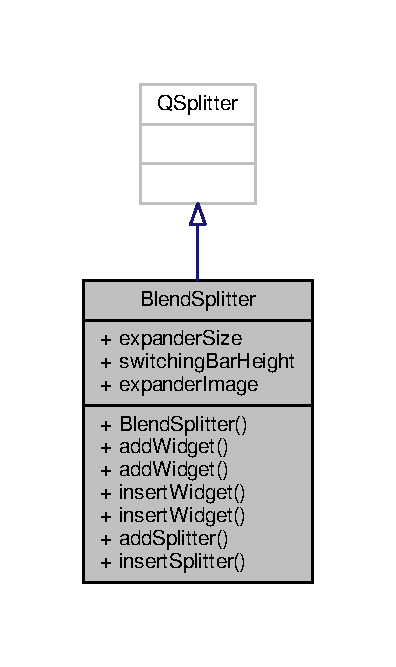
\includegraphics[width=190pt]{class_blend_splitter__inherit__graph}
\end{center}
\end{figure}


Collaboration diagram for Blend\+Splitter\+:
\nopagebreak
\begin{figure}[H]
\begin{center}
\leavevmode
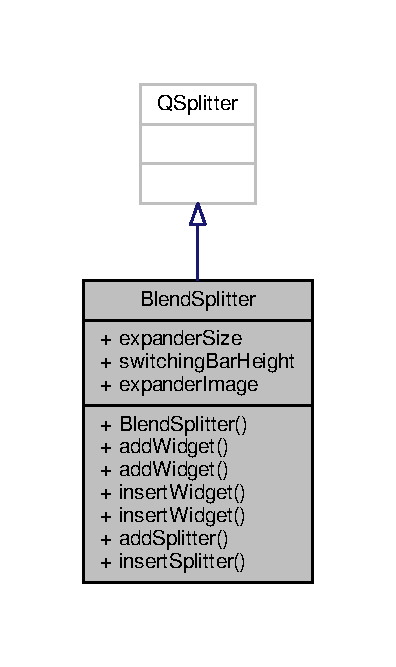
\includegraphics[width=190pt]{class_blend_splitter__coll__graph}
\end{center}
\end{figure}
\subsection*{Public Member Functions}
\begin{DoxyCompactItemize}
\item 
\hyperlink{class_blend_splitter_a8a305d92da45200aa9cc3e7160124cc3}{Blend\+Splitter} (Q\+Widget $\ast$($\ast$default\+Widget)()=\mbox{[}$\,$\mbox{]}() -\/$>$Q\+Widget $\ast$\{return new \hyperlink{class_switching_widget}{Switching\+Widget}\{\};\}, Qt\+::\+Orientation orientation=Qt\+::\+Horizontal)
\begin{DoxyCompactList}\small\item\em \hyperlink{class_blend_splitter}{Blend\+Splitter} class constructor. \end{DoxyCompactList}\item 
void \hyperlink{class_blend_splitter_a9bb010ba4ee756ca4d718acadaffb7cc}{add\+Widget} ()
\begin{DoxyCompactList}\small\item\em Add a widget to the \hyperlink{class_blend_splitter}{Blend\+Splitter}. \end{DoxyCompactList}\item 
void \hyperlink{class_blend_splitter_a305c3aee946a9fb9dcd95fdc72faff8b}{add\+Widget} (Q\+Widget $\ast$widget)
\begin{DoxyCompactList}\small\item\em Add a widget to the \hyperlink{class_blend_splitter}{Blend\+Splitter}. \end{DoxyCompactList}\item 
void \hyperlink{class_blend_splitter_a9ea589322d7bbb3e5530ad79df18a525}{add\+Widget} (\hyperlink{class_registry_item}{Registry\+Item} $\ast$item)
\begin{DoxyCompactList}\small\item\em Add a widget to the \hyperlink{class_blend_splitter}{Blend\+Splitter}. \end{DoxyCompactList}\item 
void \hyperlink{class_blend_splitter_ac26cdfb64fb785a1983a5b7527ce5189}{insert\+Widget} (int index)
\begin{DoxyCompactList}\small\item\em Insert a widget into the \hyperlink{class_blend_splitter}{Blend\+Splitter}. \end{DoxyCompactList}\item 
void \hyperlink{class_blend_splitter_a9c15101a7a0acb30f6cd46ff5259af79}{insert\+Widget} (int index, Q\+Widget $\ast$widget)
\begin{DoxyCompactList}\small\item\em Insert a widget into the \hyperlink{class_blend_splitter}{Blend\+Splitter}. \end{DoxyCompactList}\item 
void \hyperlink{class_blend_splitter_a9be82fb24eb94d1b9885cca3488e47e9}{insert\+Widget} (int index, \hyperlink{class_registry_item}{Registry\+Item} $\ast$item)
\begin{DoxyCompactList}\small\item\em Insert a widget into the \hyperlink{class_blend_splitter}{Blend\+Splitter}. \end{DoxyCompactList}\item 
void \hyperlink{class_blend_splitter_abcee5dda4bde4fdb6fda1f3c1f5b9c9a}{add\+Splitter} (\hyperlink{class_blend_splitter}{Blend\+Splitter} $\ast$splitter)
\begin{DoxyCompactList}\small\item\em Add another \hyperlink{class_blend_splitter}{Blend\+Splitter} to this \hyperlink{class_blend_splitter}{Blend\+Splitter}. \end{DoxyCompactList}\item 
void \hyperlink{class_blend_splitter_a5e1adaac62d47cc3815835e713373e2b}{insert\+Splitter} (int index, \hyperlink{class_blend_splitter}{Blend\+Splitter} $\ast$splitter)
\begin{DoxyCompactList}\small\item\em Insert another \hyperlink{class_blend_splitter}{Blend\+Splitter} into this \hyperlink{class_blend_splitter}{Blend\+Splitter}. \end{DoxyCompactList}\end{DoxyCompactItemize}
\subsection*{Static Public Attributes}
\begin{DoxyCompactItemize}
\item 
static int \hyperlink{class_blend_splitter_a233a45efce9417f826d76ce54d832d50}{expander\+Size}
\item 
static int \hyperlink{class_blend_splitter_a478fa3cfcf59f76edf8f021bee297e0d}{switching\+Bar\+Height}
\item 
static Q\+String \hyperlink{class_blend_splitter_a38c7ab0fb471718aca5eb3fe09aa124b}{expander\+Image}
\end{DoxyCompactItemize}


\subsection{Detailed Description}
A user-\/defined Splitter. 

This widget implements the functionality of Blender (Open-\/source 3D modelling software) widget management. This widget displays a splitter similar to Q\+Splitter. However, each widget in \hyperlink{class_blend_splitter}{Blend\+Splitter} has a pair of Expanders (one in top right and one in bottom left corner). By dragging from these Expanders inwards a new widget is created in the direction of the drag. If the direction is different to that of the \hyperlink{class_blend_splitter}{Blend\+Splitter}, a new \hyperlink{class_blend_splitter}{Blend\+Splitter} with parallel direction is created in place of the widget with the widget and the new widget in it. By dragging from these expanders outwards, a neighbouring widget (or a collection of widgets) can be closed. While the mouse is held, the widgets to be closed are marked with black overlay. When the mouse is released, they are closed. \hyperlink{class_blend_splitter}{Blend\+Splitter} can be used like any other Q\+Widget, although setting one as the central widget is recommended. A \hyperlink{class_blend_splitter}{Blend\+Splitter} can contain any Q\+Widget, but to achieve best results, use it together with \hyperlink{class_switching_widget}{Switching\+Widget}.

\hyperlink{class_blend_splitter}{Blend\+Splitter} provides 3 static variables that allow some customization of the library design. These are expander\+Size, switching\+Bar\+Height and expander\+Image. These are all initialized with default values. The default Expander image is provided by the library.

The default Expander image\+:



Definition at line 31 of file Blend\+Splitter.\+hpp.



\subsection{Constructor \& Destructor Documentation}
\hypertarget{class_blend_splitter_a8a305d92da45200aa9cc3e7160124cc3}{}\label{class_blend_splitter_a8a305d92da45200aa9cc3e7160124cc3} 
\index{Blend\+Splitter@{Blend\+Splitter}!Blend\+Splitter@{Blend\+Splitter}}
\index{Blend\+Splitter@{Blend\+Splitter}!Blend\+Splitter@{Blend\+Splitter}}
\subsubsection{\texorpdfstring{Blend\+Splitter()}{BlendSplitter()}}
{\footnotesize\ttfamily Blend\+Splitter\+::\+Blend\+Splitter (\begin{DoxyParamCaption}\item[{Q\+Widget $\ast$($\ast$)()}]{default\+Widget = {\ttfamily \mbox{[}\mbox{]}()~-\/$>$QWidget~$\ast$\{return~new~\hyperlink{class_switching_widget}{Switching\+Widget}\{\};\}},  }\item[{Qt\+::\+Orientation}]{orientation = {\ttfamily Qt\+:\+:Horizontal} }\end{DoxyParamCaption})}



\hyperlink{class_blend_splitter}{Blend\+Splitter} class constructor. 


\begin{DoxyParams}{Parameters}
{\em default\+Widget} & A pointer to function constructing the default widget. This function is called when a new widget is added to \hyperlink{class_blend_splitter}{Blend\+Splitter}. \\
\hline
{\em orientation} & Orientation of the main \hyperlink{class_blend_splitter}{Blend\+Splitter} \\
\hline
\end{DoxyParams}


\subsection{Member Function Documentation}
\hypertarget{class_blend_splitter_abcee5dda4bde4fdb6fda1f3c1f5b9c9a}{}\label{class_blend_splitter_abcee5dda4bde4fdb6fda1f3c1f5b9c9a} 
\index{Blend\+Splitter@{Blend\+Splitter}!add\+Splitter@{add\+Splitter}}
\index{add\+Splitter@{add\+Splitter}!Blend\+Splitter@{Blend\+Splitter}}
\subsubsection{\texorpdfstring{add\+Splitter()}{addSplitter()}}
{\footnotesize\ttfamily void Blend\+Splitter\+::add\+Splitter (\begin{DoxyParamCaption}\item[{\hyperlink{class_blend_splitter}{Blend\+Splitter} $\ast$}]{splitter }\end{DoxyParamCaption})}



Add another \hyperlink{class_blend_splitter}{Blend\+Splitter} to this \hyperlink{class_blend_splitter}{Blend\+Splitter}. 

Adds a \hyperlink{class_blend_splitter}{Blend\+Splitter} (usually with parallel orientation) to the \hyperlink{class_blend_splitter}{Blend\+Splitter} 
\begin{DoxyParams}{Parameters}
{\em splitter} & A pointer to the \hyperlink{class_blend_splitter}{Blend\+Splitter} to be added \\
\hline
\end{DoxyParams}
\hypertarget{class_blend_splitter_a9bb010ba4ee756ca4d718acadaffb7cc}{}\label{class_blend_splitter_a9bb010ba4ee756ca4d718acadaffb7cc} 
\index{Blend\+Splitter@{Blend\+Splitter}!add\+Widget@{add\+Widget}}
\index{add\+Widget@{add\+Widget}!Blend\+Splitter@{Blend\+Splitter}}
\subsubsection{\texorpdfstring{add\+Widget()}{addWidget()}\hspace{0.1cm}{\footnotesize\ttfamily [1/3]}}
{\footnotesize\ttfamily void Blend\+Splitter\+::add\+Widget (\begin{DoxyParamCaption}{ }\end{DoxyParamCaption})}



Add a widget to the \hyperlink{class_blend_splitter}{Blend\+Splitter}. 

Adds the default widget to the very bottom/right of the \hyperlink{class_blend_splitter}{Blend\+Splitter}. \hypertarget{class_blend_splitter_a305c3aee946a9fb9dcd95fdc72faff8b}{}\label{class_blend_splitter_a305c3aee946a9fb9dcd95fdc72faff8b} 
\index{Blend\+Splitter@{Blend\+Splitter}!add\+Widget@{add\+Widget}}
\index{add\+Widget@{add\+Widget}!Blend\+Splitter@{Blend\+Splitter}}
\subsubsection{\texorpdfstring{add\+Widget()}{addWidget()}\hspace{0.1cm}{\footnotesize\ttfamily [2/3]}}
{\footnotesize\ttfamily void Blend\+Splitter\+::add\+Widget (\begin{DoxyParamCaption}\item[{Q\+Widget $\ast$}]{widget }\end{DoxyParamCaption})}



Add a widget to the \hyperlink{class_blend_splitter}{Blend\+Splitter}. 

Adds the specified widget to the very bottom/right of the \hyperlink{class_blend_splitter}{Blend\+Splitter} 
\begin{DoxyParams}{Parameters}
{\em widget} & A pointer to the widget to be added \\
\hline
\end{DoxyParams}
\hypertarget{class_blend_splitter_a9ea589322d7bbb3e5530ad79df18a525}{}\label{class_blend_splitter_a9ea589322d7bbb3e5530ad79df18a525} 
\index{Blend\+Splitter@{Blend\+Splitter}!add\+Widget@{add\+Widget}}
\index{add\+Widget@{add\+Widget}!Blend\+Splitter@{Blend\+Splitter}}
\subsubsection{\texorpdfstring{add\+Widget()}{addWidget()}\hspace{0.1cm}{\footnotesize\ttfamily [3/3]}}
{\footnotesize\ttfamily void Blend\+Splitter\+::add\+Widget (\begin{DoxyParamCaption}\item[{\hyperlink{class_registry_item}{Registry\+Item} $\ast$}]{item }\end{DoxyParamCaption})}



Add a widget to the \hyperlink{class_blend_splitter}{Blend\+Splitter}. 

Adds the specified widget from the \hyperlink{class_widget_registry}{Widget\+Registry} to the very bottom/right of the \hyperlink{class_blend_splitter}{Blend\+Splitter} 
\begin{DoxyParams}{Parameters}
{\em item} & A \hyperlink{class_registry_item}{Registry\+Item} to be added (inside a \hyperlink{class_switching_widget}{Switching\+Widget}). \\
\hline
\end{DoxyParams}
\hypertarget{class_blend_splitter_a5e1adaac62d47cc3815835e713373e2b}{}\label{class_blend_splitter_a5e1adaac62d47cc3815835e713373e2b} 
\index{Blend\+Splitter@{Blend\+Splitter}!insert\+Splitter@{insert\+Splitter}}
\index{insert\+Splitter@{insert\+Splitter}!Blend\+Splitter@{Blend\+Splitter}}
\subsubsection{\texorpdfstring{insert\+Splitter()}{insertSplitter()}}
{\footnotesize\ttfamily void Blend\+Splitter\+::insert\+Splitter (\begin{DoxyParamCaption}\item[{int}]{index,  }\item[{\hyperlink{class_blend_splitter}{Blend\+Splitter} $\ast$}]{splitter }\end{DoxyParamCaption})}



Insert another \hyperlink{class_blend_splitter}{Blend\+Splitter} into this \hyperlink{class_blend_splitter}{Blend\+Splitter}. 

Inserts a \hyperlink{class_blend_splitter}{Blend\+Splitter} (usually with parallel orientation) into the \hyperlink{class_blend_splitter}{Blend\+Splitter} at the given position counting from top/left (counting starts at 0). 
\begin{DoxyParams}{Parameters}
{\em index} & The desired position \\
\hline
{\em splitter} & A pointer to the \hyperlink{class_blend_splitter}{Blend\+Splitter} to be inserted \\
\hline
\end{DoxyParams}
\hypertarget{class_blend_splitter_ac26cdfb64fb785a1983a5b7527ce5189}{}\label{class_blend_splitter_ac26cdfb64fb785a1983a5b7527ce5189} 
\index{Blend\+Splitter@{Blend\+Splitter}!insert\+Widget@{insert\+Widget}}
\index{insert\+Widget@{insert\+Widget}!Blend\+Splitter@{Blend\+Splitter}}
\subsubsection{\texorpdfstring{insert\+Widget()}{insertWidget()}\hspace{0.1cm}{\footnotesize\ttfamily [1/3]}}
{\footnotesize\ttfamily void Blend\+Splitter\+::insert\+Widget (\begin{DoxyParamCaption}\item[{int}]{index }\end{DoxyParamCaption})}



Insert a widget into the \hyperlink{class_blend_splitter}{Blend\+Splitter}. 

Inserts the default widget into the \hyperlink{class_blend_splitter}{Blend\+Splitter} at the given position counting from top/left (counting starts at 0). This function should N\+OT be called with a \hyperlink{class_blend_splitter}{Blend\+Splitter} as a parameter. 
\begin{DoxyParams}{Parameters}
{\em index} & The desired position \\
\hline
\end{DoxyParams}
\hypertarget{class_blend_splitter_a9c15101a7a0acb30f6cd46ff5259af79}{}\label{class_blend_splitter_a9c15101a7a0acb30f6cd46ff5259af79} 
\index{Blend\+Splitter@{Blend\+Splitter}!insert\+Widget@{insert\+Widget}}
\index{insert\+Widget@{insert\+Widget}!Blend\+Splitter@{Blend\+Splitter}}
\subsubsection{\texorpdfstring{insert\+Widget()}{insertWidget()}\hspace{0.1cm}{\footnotesize\ttfamily [2/3]}}
{\footnotesize\ttfamily void Blend\+Splitter\+::insert\+Widget (\begin{DoxyParamCaption}\item[{int}]{index,  }\item[{Q\+Widget $\ast$}]{widget }\end{DoxyParamCaption})}



Insert a widget into the \hyperlink{class_blend_splitter}{Blend\+Splitter}. 

Inserts the specified widget into the \hyperlink{class_blend_splitter}{Blend\+Splitter} at the given position counting from top/left (counting starts at 0). This function should N\+OT be called with a \hyperlink{class_blend_splitter}{Blend\+Splitter} as a parameter. 
\begin{DoxyParams}{Parameters}
{\em index} & The desired position \\
\hline
{\em widget} & A pointer to the widget to be inserted \\
\hline
\end{DoxyParams}
\hypertarget{class_blend_splitter_a9be82fb24eb94d1b9885cca3488e47e9}{}\label{class_blend_splitter_a9be82fb24eb94d1b9885cca3488e47e9} 
\index{Blend\+Splitter@{Blend\+Splitter}!insert\+Widget@{insert\+Widget}}
\index{insert\+Widget@{insert\+Widget}!Blend\+Splitter@{Blend\+Splitter}}
\subsubsection{\texorpdfstring{insert\+Widget()}{insertWidget()}\hspace{0.1cm}{\footnotesize\ttfamily [3/3]}}
{\footnotesize\ttfamily void Blend\+Splitter\+::insert\+Widget (\begin{DoxyParamCaption}\item[{int}]{index,  }\item[{\hyperlink{class_registry_item}{Registry\+Item} $\ast$}]{item }\end{DoxyParamCaption})}



Insert a widget into the \hyperlink{class_blend_splitter}{Blend\+Splitter}. 

Inserts the specified widget from \hyperlink{class_widget_registry}{Widget\+Registry} into the \hyperlink{class_blend_splitter}{Blend\+Splitter} at the given position counting from top/left (counting starts at 0). This function should N\+OT be called with a \hyperlink{class_blend_splitter}{Blend\+Splitter} as a parameter. 
\begin{DoxyParams}{Parameters}
{\em index} & The desired position \\
\hline
{\em item} & A \hyperlink{class_registry_item}{Registry\+Item} to be added (inside a \hyperlink{class_switching_widget}{Switching\+Widget}). \\
\hline
\end{DoxyParams}


\subsection{Member Data Documentation}
\hypertarget{class_blend_splitter_a38c7ab0fb471718aca5eb3fe09aa124b}{}\label{class_blend_splitter_a38c7ab0fb471718aca5eb3fe09aa124b} 
\index{Blend\+Splitter@{Blend\+Splitter}!expander\+Image@{expander\+Image}}
\index{expander\+Image@{expander\+Image}!Blend\+Splitter@{Blend\+Splitter}}
\subsubsection{\texorpdfstring{expander\+Image}{expanderImage}}
{\footnotesize\ttfamily Q\+String Blend\+Splitter\+::expander\+Image\hspace{0.3cm}{\ttfamily [static]}}

The image to be used for the top left expander. The bottom right one will rotate this by pi (180 degrees). Default value\+: "\+:/\+Blend\+Splitter/\+Expander" 

Definition at line 38 of file Blend\+Splitter.\+hpp.

\hypertarget{class_blend_splitter_a233a45efce9417f826d76ce54d832d50}{}\label{class_blend_splitter_a233a45efce9417f826d76ce54d832d50} 
\index{Blend\+Splitter@{Blend\+Splitter}!expander\+Size@{expander\+Size}}
\index{expander\+Size@{expander\+Size}!Blend\+Splitter@{Blend\+Splitter}}
\subsubsection{\texorpdfstring{expander\+Size}{expanderSize}}
{\footnotesize\ttfamily int Blend\+Splitter\+::expander\+Size\hspace{0.3cm}{\ttfamily [static]}}

Size of the expanders in the corners. Default value\+: 12 

Definition at line 36 of file Blend\+Splitter.\+hpp.

\hypertarget{class_blend_splitter_a478fa3cfcf59f76edf8f021bee297e0d}{}\label{class_blend_splitter_a478fa3cfcf59f76edf8f021bee297e0d} 
\index{Blend\+Splitter@{Blend\+Splitter}!switching\+Bar\+Height@{switching\+Bar\+Height}}
\index{switching\+Bar\+Height@{switching\+Bar\+Height}!Blend\+Splitter@{Blend\+Splitter}}
\subsubsection{\texorpdfstring{switching\+Bar\+Height}{switchingBarHeight}}
{\footnotesize\ttfamily int Blend\+Splitter\+::switching\+Bar\+Height\hspace{0.3cm}{\ttfamily [static]}}

Height of the \hyperlink{class_switching_bar}{Switching\+Bar}. Default value\+: 36 

Definition at line 37 of file Blend\+Splitter.\+hpp.



The documentation for this class was generated from the following file\+:\begin{DoxyCompactItemize}
\item 
include/Blend\+Splitter.\+hpp\end{DoxyCompactItemize}

\hypertarget{class_registry_item}{}\section{Registry\+Item Class Reference}
\label{class_registry_item}\index{Registry\+Item@{Registry\+Item}}


An item intended to be put into \hyperlink{class_widget_registry}{Widget\+Registry}.  




{\ttfamily \#include $<$Registry\+Item.\+hpp$>$}



Collaboration diagram for Registry\+Item\+:
\nopagebreak
\begin{figure}[H]
\begin{center}
\leavevmode
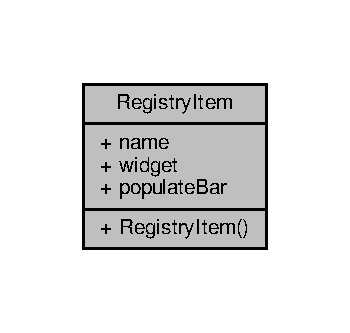
\includegraphics[width=168pt]{class_registry_item__coll__graph}
\end{center}
\end{figure}
\subsection*{Public Member Functions}
\begin{DoxyCompactItemize}
\item 
\hyperlink{class_registry_item_a6a4c02c5562dc8cbc61bee94f7a8db49}{Registry\+Item} (Q\+String \hyperlink{class_registry_item_a662d7e2c473bea72a0549caf63ea5bfd}{name}=\char`\"{}Default\char`\"{}, Q\+Widget $\ast$($\ast$\hyperlink{class_registry_item_aa95c5a5dbfdf491e53b07dbc0a027e14}{widget})()=\mbox{[}$\,$\mbox{]}() -\/$>$Q\+Widget $\ast$\{return new Q\+Label\{\char`\"{}Default Widget\char`\"{}\};\}, void($\ast$\hyperlink{class_registry_item_a0784869b48c86a581e12c88fd2706cd0}{populate\+Bar})(\hyperlink{class_switching_bar}{Switching\+Bar} $\ast$, Q\+Widget $\ast$)=\mbox{[}$\,$\mbox{]}(\hyperlink{class_switching_bar}{Switching\+Bar} $\ast$, Q\+Widget $\ast$) -\/$>$void \{\})
\begin{DoxyCompactList}\small\item\em A constructor setting all the internal values. \end{DoxyCompactList}\end{DoxyCompactItemize}
\subsection*{Public Attributes}
\begin{DoxyCompactItemize}
\item 
Q\+String \hyperlink{class_registry_item_a662d7e2c473bea72a0549caf63ea5bfd}{name}
\item 
Q\+Widget $\ast$($\ast$ \hyperlink{class_registry_item_aa95c5a5dbfdf491e53b07dbc0a027e14}{widget} )()
\begin{DoxyCompactList}\small\item\em A function constructing the widget. \end{DoxyCompactList}\item 
void($\ast$ \hyperlink{class_registry_item_a0784869b48c86a581e12c88fd2706cd0}{populate\+Bar} )(\hyperlink{class_switching_bar}{Switching\+Bar} $\ast$, Q\+Widget $\ast$)
\begin{DoxyCompactList}\small\item\em A function populating the \hyperlink{class_switching_bar}{Switching\+Bar}. \end{DoxyCompactList}\end{DoxyCompactItemize}


\subsection{Detailed Description}
An item intended to be put into \hyperlink{class_widget_registry}{Widget\+Registry}. 

Each \hyperlink{class_registry_item}{Registry\+Item} corresponds to one widget that can be displayed in a \hyperlink{class_blend_splitter}{Blend\+Splitter}. It describes how this widget should be constructed, what is its name and what items should be in the \hyperlink{class_switching_bar}{Switching\+Bar} when this widget is selected. 

Definition at line 17 of file Registry\+Item.\+hpp.



\subsection{Constructor \& Destructor Documentation}
\hypertarget{class_registry_item_a6a4c02c5562dc8cbc61bee94f7a8db49}{}\label{class_registry_item_a6a4c02c5562dc8cbc61bee94f7a8db49} 
\index{Registry\+Item@{Registry\+Item}!Registry\+Item@{Registry\+Item}}
\index{Registry\+Item@{Registry\+Item}!Registry\+Item@{Registry\+Item}}
\subsubsection{\texorpdfstring{Registry\+Item()}{RegistryItem()}}
{\footnotesize\ttfamily Registry\+Item\+::\+Registry\+Item (\begin{DoxyParamCaption}\item[{Q\+String}]{name = {\ttfamily \char`\"{}Default\char`\"{}},  }\item[{Q\+Widget $\ast$($\ast$)()}]{widget = {\ttfamily \mbox{[}\mbox{]}()~-\/$>$QWidget~$\ast$\{return~new~QLabel\{\char`\"{}Default~Widget\char`\"{}\};\}},  }\item[{void($\ast$)(\hyperlink{class_switching_bar}{Switching\+Bar} $\ast$, Q\+Widget $\ast$)}]{populate\+Bar = {\ttfamily \mbox{[}\mbox{]}(\hyperlink{class_switching_bar}{Switching\+Bar}~$\ast$,~QWidget~$\ast$)~-\/$>$void~\{\}} }\end{DoxyParamCaption})}



A constructor setting all the internal values. 

This constructor takes 3 parameters corresponding to the 3 members of the \hyperlink{class_registry_item}{Registry\+Item} class. See their desription for more details. 
\begin{DoxyParams}{Parameters}
{\em name} & The name of the widget, used in the \hyperlink{class_switching_bar}{Switching\+Bar} combo box \\
\hline
{\em widget} & A pointer to a function constructing the widget \\
\hline
{\em populate\+Bar} & A pointer to a function populating the \hyperlink{class_switching_bar}{Switching\+Bar} \\
\hline
\end{DoxyParams}


\subsection{Member Data Documentation}
\hypertarget{class_registry_item_a662d7e2c473bea72a0549caf63ea5bfd}{}\label{class_registry_item_a662d7e2c473bea72a0549caf63ea5bfd} 
\index{Registry\+Item@{Registry\+Item}!name@{name}}
\index{name@{name}!Registry\+Item@{Registry\+Item}}
\subsubsection{\texorpdfstring{name}{name}}
{\footnotesize\ttfamily Q\+String Registry\+Item\+::name}

The name of the widget, used in the \hyperlink{class_switching_bar}{Switching\+Bar} combo box. 

Definition at line 20 of file Registry\+Item.\+hpp.

\hypertarget{class_registry_item_a0784869b48c86a581e12c88fd2706cd0}{}\label{class_registry_item_a0784869b48c86a581e12c88fd2706cd0} 
\index{Registry\+Item@{Registry\+Item}!populate\+Bar@{populate\+Bar}}
\index{populate\+Bar@{populate\+Bar}!Registry\+Item@{Registry\+Item}}
\subsubsection{\texorpdfstring{populate\+Bar}{populateBar}}
{\footnotesize\ttfamily void($\ast$ Registry\+Item\+::populate\+Bar) (\hyperlink{class_switching_bar}{Switching\+Bar} $\ast$, Q\+Widget $\ast$)}



A function populating the \hyperlink{class_switching_bar}{Switching\+Bar}. 

A pointer to a function populating the \hyperlink{class_switching_bar}{Switching\+Bar}. This function is called each time this widget is selected in any \hyperlink{class_switching_widget}{Switching\+Widget}. Usually this function makes use of the interface provided by \hyperlink{class_switching_bar}{Switching\+Bar} to populate it. 
\begin{DoxyParams}{Parameters}
{\em A} & pointer to the \hyperlink{class_switching_bar}{Switching\+Bar} to be populated \\
\hline
{\em A} & pointer to the newly-\/created widget in the \hyperlink{class_switching_widget}{Switching\+Widget} \\
\hline
\end{DoxyParams}


Definition at line 33 of file Registry\+Item.\+hpp.

\hypertarget{class_registry_item_aa95c5a5dbfdf491e53b07dbc0a027e14}{}\label{class_registry_item_aa95c5a5dbfdf491e53b07dbc0a027e14} 
\index{Registry\+Item@{Registry\+Item}!widget@{widget}}
\index{widget@{widget}!Registry\+Item@{Registry\+Item}}
\subsubsection{\texorpdfstring{widget}{widget}}
{\footnotesize\ttfamily Q\+Widget$\ast$($\ast$ Registry\+Item\+::widget) ()}



A function constructing the widget. 

A pointer to a function returning Q\+Widget$\ast$. This function is called to construct the widget each time it is selected in any \hyperlink{class_switching_widget}{Switching\+Widget}. Usually in this function the widget is dynamically created using {\ttfamily new} operator and the pointer is returned. \begin{DoxyReturn}{Returns}
A pointer to the newly-\/created Q\+Widget 
\end{DoxyReturn}


Definition at line 26 of file Registry\+Item.\+hpp.



The documentation for this class was generated from the following file\+:\begin{DoxyCompactItemize}
\item 
include/\+B\+S/Registry\+Item.\+hpp\end{DoxyCompactItemize}

\hypertarget{class_switching_bar}{}\section{Switching\+Bar Class Reference}
\label{class_switching_bar}\index{Switching\+Bar@{Switching\+Bar}}


A menu bar which is always found on the bottom of \hyperlink{class_switching_widget}{Switching\+Widget}.  




{\ttfamily \#include $<$Switching\+Bar.\+hpp$>$}



Inheritance diagram for Switching\+Bar\+:
\nopagebreak
\begin{figure}[H]
\begin{center}
\leavevmode
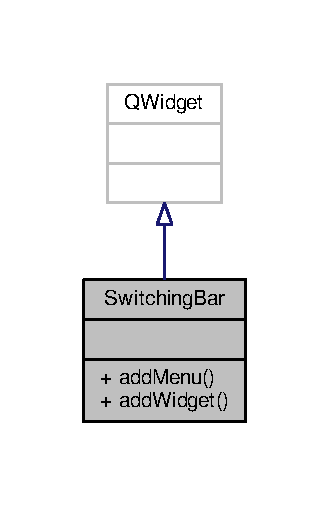
\includegraphics[width=158pt]{class_switching_bar__inherit__graph}
\end{center}
\end{figure}


Collaboration diagram for Switching\+Bar\+:
\nopagebreak
\begin{figure}[H]
\begin{center}
\leavevmode
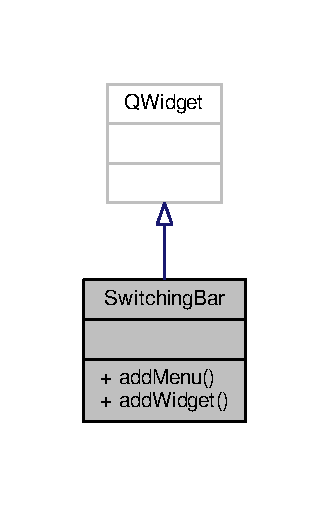
\includegraphics[width=158pt]{class_switching_bar__coll__graph}
\end{center}
\end{figure}
\subsection*{Public Member Functions}
\begin{DoxyCompactItemize}
\item 
void \hyperlink{class_switching_bar_ad92ca7f8533cb2a9993b30b49126a2b4}{add\+Menu} (Q\+Menu $\ast$menu)
\begin{DoxyCompactList}\small\item\em Add a Q\+Menu. \end{DoxyCompactList}\item 
void \hyperlink{class_switching_bar_a8e30709aa4ada4364acf8b755f8eefb6}{add\+Widget} (Q\+Widget $\ast$widget)
\begin{DoxyCompactList}\small\item\em Add a Q\+Widget. \end{DoxyCompactList}\end{DoxyCompactItemize}


\subsection{Detailed Description}
A menu bar which is always found on the bottom of \hyperlink{class_switching_widget}{Switching\+Widget}. 

This menu bar is similar to the built-\/in Q\+Menu\+Bar, but can also contain plain Q\+Widgets. The first item on the left is always a combo box for selecting which widget should be displayed in the \hyperlink{class_switching_widget}{Switching\+Widget}. 

Definition at line 20 of file Switching\+Bar.\+hpp.



\subsection{Member Function Documentation}
\hypertarget{class_switching_bar_ad92ca7f8533cb2a9993b30b49126a2b4}{}\label{class_switching_bar_ad92ca7f8533cb2a9993b30b49126a2b4} 
\index{Switching\+Bar@{Switching\+Bar}!add\+Menu@{add\+Menu}}
\index{add\+Menu@{add\+Menu}!Switching\+Bar@{Switching\+Bar}}
\subsubsection{\texorpdfstring{add\+Menu()}{addMenu()}}
{\footnotesize\ttfamily void Switching\+Bar\+::add\+Menu (\begin{DoxyParamCaption}\item[{Q\+Menu $\ast$}]{menu }\end{DoxyParamCaption})}



Add a Q\+Menu. 

This function adds a Q\+Menu to the very right of the \hyperlink{class_switching_bar}{Switching\+Bar}. The menu is wrapped in an invisible Q\+Menu\+Bar. 
\begin{DoxyParams}{Parameters}
{\em menu} & A pointer to the Q\+Menu to be added \\
\hline
\end{DoxyParams}
\hypertarget{class_switching_bar_a8e30709aa4ada4364acf8b755f8eefb6}{}\label{class_switching_bar_a8e30709aa4ada4364acf8b755f8eefb6} 
\index{Switching\+Bar@{Switching\+Bar}!add\+Widget@{add\+Widget}}
\index{add\+Widget@{add\+Widget}!Switching\+Bar@{Switching\+Bar}}
\subsubsection{\texorpdfstring{add\+Widget()}{addWidget()}}
{\footnotesize\ttfamily void Switching\+Bar\+::add\+Widget (\begin{DoxyParamCaption}\item[{Q\+Widget $\ast$}]{widget }\end{DoxyParamCaption})}



Add a Q\+Widget. 

This function adds a Q\+Widget to the very right of the \hyperlink{class_switching_bar}{Switching\+Bar}. The widget is placed in a Q\+H\+Box\+Layout. 
\begin{DoxyParams}{Parameters}
{\em widget} & A pointer to the Q\+Widget to be added \\
\hline
\end{DoxyParams}


The documentation for this class was generated from the following file\+:\begin{DoxyCompactItemize}
\item 
include/\+B\+S/Switching\+Bar.\+hpp\end{DoxyCompactItemize}

\hypertarget{class_switching_widget}{}\section{Switching\+Widget Class Reference}
\label{class_switching_widget}\index{Switching\+Widget@{Switching\+Widget}}


A widget whose actual content can be selected from a combo box.  




{\ttfamily \#include $<$Switching\+Widget.\+hpp$>$}



Inheritance diagram for Switching\+Widget\+:
\nopagebreak
\begin{figure}[H]
\begin{center}
\leavevmode
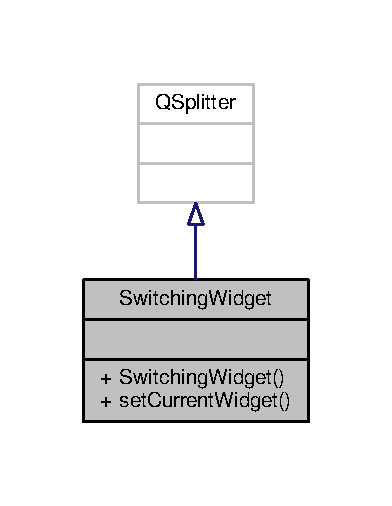
\includegraphics[width=185pt]{class_switching_widget__inherit__graph}
\end{center}
\end{figure}


Collaboration diagram for Switching\+Widget\+:
\nopagebreak
\begin{figure}[H]
\begin{center}
\leavevmode
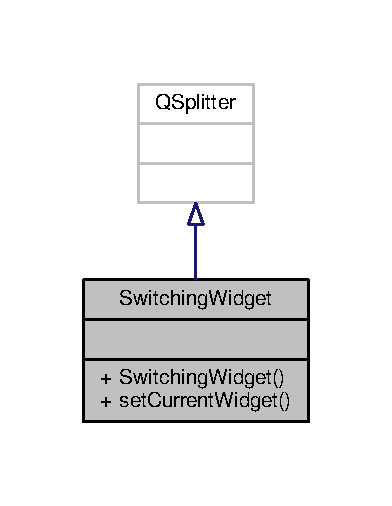
\includegraphics[width=185pt]{class_switching_widget__coll__graph}
\end{center}
\end{figure}
\subsection*{Public Member Functions}
\begin{DoxyCompactItemize}
\item 
\hyperlink{class_switching_widget_a27023a20084bccbe3095c8a4bbed8115}{Switching\+Widget} (Q\+Widget $\ast$parent=nullptr)
\begin{DoxyCompactList}\small\item\em A default constructor similar to that of Q\+Widget. \end{DoxyCompactList}\end{DoxyCompactItemize}


\subsection{Detailed Description}
A widget whose actual content can be selected from a combo box. 

This widget displays a Widget with a \hyperlink{class_switching_bar}{Switching\+Bar} on the bottom. The widget displayed is one from \hyperlink{class_widget_registry}{Widget\+Registry} and it can be selected using a combo box in the \hyperlink{class_switching_bar}{Switching\+Bar}. 

Definition at line 17 of file Switching\+Widget.\+hpp.



\subsection{Constructor \& Destructor Documentation}
\index{Switching\+Widget@{Switching\+Widget}!Switching\+Widget@{Switching\+Widget}}
\index{Switching\+Widget@{Switching\+Widget}!Switching\+Widget@{Switching\+Widget}}
\subsubsection[{\texorpdfstring{Switching\+Widget(\+Q\+Widget $\ast$parent=nullptr)}{SwitchingWidget(QWidget *parent=nullptr)}}]{\setlength{\rightskip}{0pt plus 5cm}Switching\+Widget\+::\+Switching\+Widget (
\begin{DoxyParamCaption}
\item[{Q\+Widget $\ast$}]{parent = {\ttfamily nullptr}}
\end{DoxyParamCaption}
)\hspace{0.3cm}{\ttfamily [explicit]}}\hypertarget{class_switching_widget_a27023a20084bccbe3095c8a4bbed8115}{}\label{class_switching_widget_a27023a20084bccbe3095c8a4bbed8115}


A default constructor similar to that of Q\+Widget. 

Creates a \hyperlink{class_switching_widget}{Switching\+Widget} containg the default widget specified in \hyperlink{class_widget_registry}{Widget\+Registry} 
\begin{DoxyParams}{Parameters}
{\em parent} & A parent widget \\
\hline
\end{DoxyParams}


The documentation for this class was generated from the following file\+:\begin{DoxyCompactItemize}
\item 
include/\+B\+S/Switching\+Widget.\+hpp\end{DoxyCompactItemize}

\hypertarget{class_widget_registry}{}\section{Widget\+Registry Class Reference}
\label{class_widget_registry}\index{Widget\+Registry@{Widget\+Registry}}


A registry of all widgets that can be displayed in a \hyperlink{class_switching_widget}{Switching\+Widget}.  




{\ttfamily \#include $<$Widget\+Registry.\+hpp$>$}



Inheritance diagram for Widget\+Registry\+:
\nopagebreak
\begin{figure}[H]
\begin{center}
\leavevmode
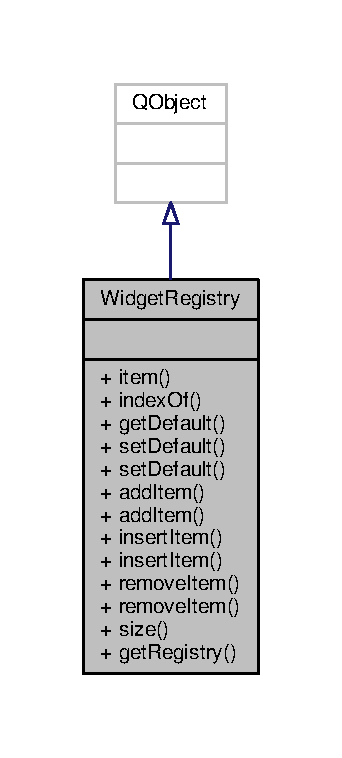
\includegraphics[width=164pt]{class_widget_registry__inherit__graph}
\end{center}
\end{figure}


Collaboration diagram for Widget\+Registry\+:
\nopagebreak
\begin{figure}[H]
\begin{center}
\leavevmode
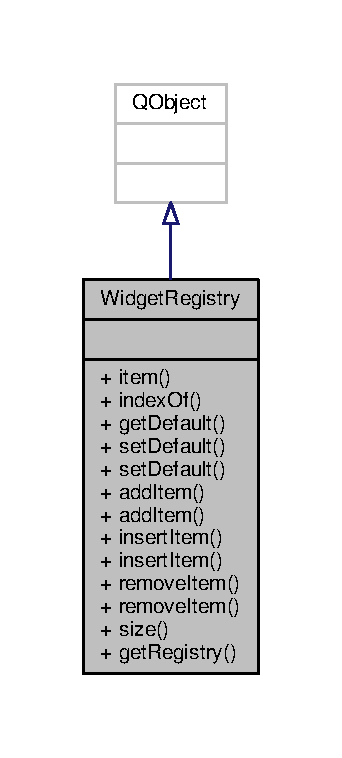
\includegraphics[width=164pt]{class_widget_registry__coll__graph}
\end{center}
\end{figure}
\subsection*{Signals}
\begin{DoxyCompactItemize}
\item 
void \hyperlink{class_widget_registry_aaf17eb75aaf18be5094dfd96f2d96fcc}{registry\+Changed} ()
\begin{DoxyCompactList}\small\item\em Signal emited when \hyperlink{class_widget_registry}{Widget\+Registry} changes its contents. \end{DoxyCompactList}\end{DoxyCompactItemize}
\subsection*{Public Member Functions}
\begin{DoxyCompactItemize}
\item 
\hyperlink{class_registry_item}{Registry\+Item} $\ast$ \hyperlink{class_widget_registry_a432f0e1f366c3d5dce760e83fd8260fe}{item} (int i) const
\begin{DoxyCompactList}\small\item\em Get the item at position i. \end{DoxyCompactList}\item 
int \hyperlink{class_widget_registry_aa0855242e9b8aa7ec76cace984c26e57}{index\+Of} (\hyperlink{class_registry_item}{Registry\+Item} $\ast$\hyperlink{class_widget_registry_a432f0e1f366c3d5dce760e83fd8260fe}{item}) const
\begin{DoxyCompactList}\small\item\em Get the position of an item in \hyperlink{class_widget_registry}{Widget\+Registry}. \end{DoxyCompactList}\item 
\hyperlink{class_registry_item}{Registry\+Item} $\ast$ \hyperlink{class_widget_registry_a0841639b77ada4dc770886fea9fef193}{get\+Default} ()
\begin{DoxyCompactList}\small\item\em Get the default \hyperlink{class_registry_item}{Registry\+Item}. \end{DoxyCompactList}\item 
void \hyperlink{class_widget_registry_aa77ed2504c7e241eabf49ff4e1088fa2}{set\+Default} (\hyperlink{class_registry_item}{Registry\+Item} $\ast$\hyperlink{class_widget_registry_a432f0e1f366c3d5dce760e83fd8260fe}{item})
\begin{DoxyCompactList}\small\item\em Set the default \hyperlink{class_registry_item}{Registry\+Item}. \end{DoxyCompactList}\item 
void \hyperlink{class_widget_registry_a3d0fa9207009556d5218a3dda73349d0}{set\+Default} (int index=0)
\begin{DoxyCompactList}\small\item\em Set the default \hyperlink{class_registry_item}{Registry\+Item}. \end{DoxyCompactList}\item 
void \hyperlink{class_widget_registry_a53de88d7a538a8a6bbbcca4328abb480}{add\+Item} (\hyperlink{class_registry_item}{Registry\+Item} $\ast$\hyperlink{class_widget_registry_a432f0e1f366c3d5dce760e83fd8260fe}{item})
\begin{DoxyCompactList}\small\item\em Add an item to \hyperlink{class_widget_registry}{Widget\+Registry}. \end{DoxyCompactList}\item 
void \hyperlink{class_widget_registry_a545df9d9afbcfa625795cb7d2834aac5}{add\+Item} (Q\+String name=\char`\"{}Default\char`\"{}, Q\+Widget $\ast$($\ast$widget)()=\mbox{[}$\,$\mbox{]}() -\/$>$Q\+Widget $\ast$\{return new Q\+Label\{\char`\"{}Default widget\char`\"{}\};\}, void($\ast$populate\+Bar)(\hyperlink{class_switching_bar}{Switching\+Bar} $\ast$, Q\+Widget $\ast$)=\mbox{[}$\,$\mbox{]}(\hyperlink{class_switching_bar}{Switching\+Bar} $\ast$, Q\+Widget $\ast$) -\/$>$void \{\})
\begin{DoxyCompactList}\small\item\em Add an item to \hyperlink{class_widget_registry}{Widget\+Registry}. \end{DoxyCompactList}\item 
void \hyperlink{class_widget_registry_a3a323a51d1e65d61d6ed9b8639a21070}{insert\+Item} (int index, \hyperlink{class_registry_item}{Registry\+Item} $\ast$\hyperlink{class_widget_registry_a432f0e1f366c3d5dce760e83fd8260fe}{item})
\begin{DoxyCompactList}\small\item\em Insert an item into \hyperlink{class_widget_registry}{Widget\+Registry}. \end{DoxyCompactList}\item 
void \hyperlink{class_widget_registry_ac39d282b5e1639e3e9a3e0dfdae8e92e}{insert\+Item} (int index, Q\+String name=\char`\"{}Default\char`\"{}, Q\+Widget $\ast$($\ast$widget)()=\mbox{[}$\,$\mbox{]}() -\/$>$Q\+Widget $\ast$\{return new Q\+Label\{\char`\"{}Default widget\char`\"{}\};\}, void($\ast$populate\+Bar)(\hyperlink{class_switching_bar}{Switching\+Bar} $\ast$, Q\+Widget $\ast$)=\mbox{[}$\,$\mbox{]}(\hyperlink{class_switching_bar}{Switching\+Bar} $\ast$, Q\+Widget $\ast$) -\/$>$void \{\})
\begin{DoxyCompactList}\small\item\em Insert an item into widget\+Registry. \end{DoxyCompactList}\item 
void \hyperlink{class_widget_registry_a076561002958c840a9096d27cdbfdeed}{remove\+Item} (\hyperlink{class_registry_item}{Registry\+Item} $\ast$\hyperlink{class_widget_registry_a432f0e1f366c3d5dce760e83fd8260fe}{item})
\begin{DoxyCompactList}\small\item\em Remove a \hyperlink{class_registry_item}{Registry\+Item} from \hyperlink{class_widget_registry}{Widget\+Registry}. \end{DoxyCompactList}\item 
void \hyperlink{class_widget_registry_a96abefe3fed38e9424609cc3cf2f8d7d}{remove\+Item} (int index)
\begin{DoxyCompactList}\small\item\em Remove a \hyperlink{class_registry_item}{Registry\+Item} from \hyperlink{class_widget_registry}{Widget\+Registry}. \end{DoxyCompactList}\item 
int \hyperlink{class_widget_registry_a13ca89bca85a4680f79e56d29263d219}{size} () const
\begin{DoxyCompactList}\small\item\em Get the size of \hyperlink{class_widget_registry}{Widget\+Registry}. \end{DoxyCompactList}\end{DoxyCompactItemize}
\subsection*{Static Public Member Functions}
\begin{DoxyCompactItemize}
\item 
static \hyperlink{class_widget_registry}{Widget\+Registry} $\ast$ \hyperlink{class_widget_registry_ad0c8eaf65a4c00947866a56cc2c48eb2}{get\+Registry} ()
\begin{DoxyCompactList}\small\item\em Registry getter. \end{DoxyCompactList}\end{DoxyCompactItemize}


\subsection{Detailed Description}
A registry of all widgets that can be displayed in a \hyperlink{class_switching_widget}{Switching\+Widget}. 

This singleton-\/class acts as a registry of widgets that can be displayed in a \hyperlink{class_switching_widget}{Switching\+Widget} by selecting from a combo box in the \hyperlink{class_switching_bar}{Switching\+Bar}. Each item is represented as one \hyperlink{class_registry_item}{Registry\+Item}. The Registry also contains a pointer to the default \hyperlink{class_registry_item}{Registry\+Item}, which is shown when a new \hyperlink{class_switching_widget}{Switching\+Widget} is created. 

Definition at line 18 of file Widget\+Registry.\+hpp.



\subsection{Member Function Documentation}
\hypertarget{class_widget_registry_a53de88d7a538a8a6bbbcca4328abb480}{}\label{class_widget_registry_a53de88d7a538a8a6bbbcca4328abb480} 
\index{Widget\+Registry@{Widget\+Registry}!add\+Item@{add\+Item}}
\index{add\+Item@{add\+Item}!Widget\+Registry@{Widget\+Registry}}
\subsubsection{\texorpdfstring{add\+Item()}{addItem()}\hspace{0.1cm}{\footnotesize\ttfamily [1/2]}}
{\footnotesize\ttfamily void Widget\+Registry\+::add\+Item (\begin{DoxyParamCaption}\item[{\hyperlink{class_registry_item}{Registry\+Item} $\ast$}]{item }\end{DoxyParamCaption})}



Add an item to \hyperlink{class_widget_registry}{Widget\+Registry}. 

Adds a given \hyperlink{class_registry_item}{Registry\+Item} at the end of \hyperlink{class_widget_registry}{Widget\+Registry}. 
\begin{DoxyParams}{Parameters}
{\em item} & A pointer to the \hyperlink{class_registry_item}{Registry\+Item} to be added \\
\hline
\end{DoxyParams}
\hypertarget{class_widget_registry_a545df9d9afbcfa625795cb7d2834aac5}{}\label{class_widget_registry_a545df9d9afbcfa625795cb7d2834aac5} 
\index{Widget\+Registry@{Widget\+Registry}!add\+Item@{add\+Item}}
\index{add\+Item@{add\+Item}!Widget\+Registry@{Widget\+Registry}}
\subsubsection{\texorpdfstring{add\+Item()}{addItem()}\hspace{0.1cm}{\footnotesize\ttfamily [2/2]}}
{\footnotesize\ttfamily void Widget\+Registry\+::add\+Item (\begin{DoxyParamCaption}\item[{Q\+String}]{name = {\ttfamily \char`\"{}Default\char`\"{}},  }\item[{Q\+Widget $\ast$($\ast$)()}]{widget = {\ttfamily \mbox{[}\mbox{]}()~-\/$>$QWidget~$\ast$\{return~new~QLabel\{\char`\"{}Default~widget\char`\"{}\};\}},  }\item[{void($\ast$)(\hyperlink{class_switching_bar}{Switching\+Bar} $\ast$, Q\+Widget $\ast$)}]{populate\+Bar = {\ttfamily \mbox{[}\mbox{]}(\hyperlink{class_switching_bar}{Switching\+Bar}~$\ast$,~QWidget~$\ast$)~-\/$>$void~\{\}} }\end{DoxyParamCaption})}



Add an item to \hyperlink{class_widget_registry}{Widget\+Registry}. 

Adds a \hyperlink{class_registry_item}{Registry\+Item} constructed with the given parameters at the end of \hyperlink{class_widget_registry}{Widget\+Registry}. This is equal to calling add\+Item(new \hyperlink{class_registry_item}{Registry\+Item}\{name, widget, populate\+Bar\}). 
\begin{DoxyParams}{Parameters}
{\em name} & The name of the widget, used in the \hyperlink{class_switching_bar}{Switching\+Bar} combo box \\
\hline
{\em widget} & A pointer to a function constructing the widget \\
\hline
{\em populate\+Bar} & A pointer to a function populating the \hyperlink{class_switching_bar}{Switching\+Bar} \\
\hline
\end{DoxyParams}
\hypertarget{class_widget_registry_a0841639b77ada4dc770886fea9fef193}{}\label{class_widget_registry_a0841639b77ada4dc770886fea9fef193} 
\index{Widget\+Registry@{Widget\+Registry}!get\+Default@{get\+Default}}
\index{get\+Default@{get\+Default}!Widget\+Registry@{Widget\+Registry}}
\subsubsection{\texorpdfstring{get\+Default()}{getDefault()}}
{\footnotesize\ttfamily \hyperlink{class_registry_item}{Registry\+Item}$\ast$ Widget\+Registry\+::get\+Default (\begin{DoxyParamCaption}{ }\end{DoxyParamCaption})}



Get the default \hyperlink{class_registry_item}{Registry\+Item}. 

This function gives you the default \hyperlink{class_registry_item}{Registry\+Item}. Note that if no item was set as default, the currently first item is set as default by this function. If the registry is empty, a \hyperlink{class_registry_item}{Registry\+Item} is added to the registry (using the default constructor) and set as default. \begin{DoxyReturn}{Returns}
A pointer to the default \hyperlink{class_registry_item}{Registry\+Item} 
\end{DoxyReturn}
\hypertarget{class_widget_registry_ad0c8eaf65a4c00947866a56cc2c48eb2}{}\label{class_widget_registry_ad0c8eaf65a4c00947866a56cc2c48eb2} 
\index{Widget\+Registry@{Widget\+Registry}!get\+Registry@{get\+Registry}}
\index{get\+Registry@{get\+Registry}!Widget\+Registry@{Widget\+Registry}}
\subsubsection{\texorpdfstring{get\+Registry()}{getRegistry()}}
{\footnotesize\ttfamily static \hyperlink{class_widget_registry}{Widget\+Registry}$\ast$ Widget\+Registry\+::get\+Registry (\begin{DoxyParamCaption}{ }\end{DoxyParamCaption})\hspace{0.3cm}{\ttfamily [static]}}



Registry getter. 

This is a singleton class, i. e. you can\textquotesingle{}t construct any object yourself. To get the one-\/and-\/only instance of this class, you need to call \hyperlink{class_widget_registry_ad0c8eaf65a4c00947866a56cc2c48eb2}{Widget\+Registry\+::get\+Registry()}. The function will create the object if neccessary (= when called for the first time) and return a pointer to it. \begin{DoxyReturn}{Returns}
A pointer to the one-\/and-\/only instance of \hyperlink{class_widget_registry}{Widget\+Registry} 
\end{DoxyReturn}
\hypertarget{class_widget_registry_aa0855242e9b8aa7ec76cace984c26e57}{}\label{class_widget_registry_aa0855242e9b8aa7ec76cace984c26e57} 
\index{Widget\+Registry@{Widget\+Registry}!index\+Of@{index\+Of}}
\index{index\+Of@{index\+Of}!Widget\+Registry@{Widget\+Registry}}
\subsubsection{\texorpdfstring{index\+Of()}{indexOf()}}
{\footnotesize\ttfamily int Widget\+Registry\+::index\+Of (\begin{DoxyParamCaption}\item[{\hyperlink{class_registry_item}{Registry\+Item} $\ast$}]{item }\end{DoxyParamCaption}) const}



Get the position of an item in \hyperlink{class_widget_registry}{Widget\+Registry}. 

Get the index (counting starts at 0) of an item. Often used together with \hyperlink{class_widget_registry_a432f0e1f366c3d5dce760e83fd8260fe}{item(int i) const}. 
\begin{DoxyParams}{Parameters}
{\em item} & A pointer to the item whose index is to be returned \\
\hline
\end{DoxyParams}
\begin{DoxyReturn}{Returns}
Index of the item 
\end{DoxyReturn}
\hypertarget{class_widget_registry_a3a323a51d1e65d61d6ed9b8639a21070}{}\label{class_widget_registry_a3a323a51d1e65d61d6ed9b8639a21070} 
\index{Widget\+Registry@{Widget\+Registry}!insert\+Item@{insert\+Item}}
\index{insert\+Item@{insert\+Item}!Widget\+Registry@{Widget\+Registry}}
\subsubsection{\texorpdfstring{insert\+Item()}{insertItem()}\hspace{0.1cm}{\footnotesize\ttfamily [1/2]}}
{\footnotesize\ttfamily void Widget\+Registry\+::insert\+Item (\begin{DoxyParamCaption}\item[{int}]{index,  }\item[{\hyperlink{class_registry_item}{Registry\+Item} $\ast$}]{item }\end{DoxyParamCaption})}



Insert an item into \hyperlink{class_widget_registry}{Widget\+Registry}. 

Inserts a given \hyperlink{class_registry_item}{Registry\+Item} into \hyperlink{class_widget_registry}{Widget\+Registry} at a given index. 
\begin{DoxyParams}{Parameters}
{\em index} & The desired index of the inserted \hyperlink{class_registry_item}{Registry\+Item} (counting starts at 0) \\
\hline
{\em item} & A pointer to the \hyperlink{class_registry_item}{Registry\+Item} to be added \\
\hline
\end{DoxyParams}
\hypertarget{class_widget_registry_ac39d282b5e1639e3e9a3e0dfdae8e92e}{}\label{class_widget_registry_ac39d282b5e1639e3e9a3e0dfdae8e92e} 
\index{Widget\+Registry@{Widget\+Registry}!insert\+Item@{insert\+Item}}
\index{insert\+Item@{insert\+Item}!Widget\+Registry@{Widget\+Registry}}
\subsubsection{\texorpdfstring{insert\+Item()}{insertItem()}\hspace{0.1cm}{\footnotesize\ttfamily [2/2]}}
{\footnotesize\ttfamily void Widget\+Registry\+::insert\+Item (\begin{DoxyParamCaption}\item[{int}]{index,  }\item[{Q\+String}]{name = {\ttfamily \char`\"{}Default\char`\"{}},  }\item[{Q\+Widget $\ast$($\ast$)()}]{widget = {\ttfamily \mbox{[}\mbox{]}()~-\/$>$QWidget~$\ast$\{return~new~QLabel\{\char`\"{}Default~widget\char`\"{}\};\}},  }\item[{void($\ast$)(\hyperlink{class_switching_bar}{Switching\+Bar} $\ast$, Q\+Widget $\ast$)}]{populate\+Bar = {\ttfamily \mbox{[}\mbox{]}(\hyperlink{class_switching_bar}{Switching\+Bar}~$\ast$,~QWidget~$\ast$)~-\/$>$void~\{\}} }\end{DoxyParamCaption})}



Insert an item into widget\+Registry. 

Inserts a \hyperlink{class_registry_item}{Registry\+Item} constructed with the given parameters into \hyperlink{class_widget_registry}{Widget\+Registry} at a given index. This is equal to calling insert\+Item(index, new \hyperlink{class_registry_item}{Registry\+Item}\{name, widget, populate\+Bar\}). 
\begin{DoxyParams}{Parameters}
{\em index} & The desired index of the inserted \hyperlink{class_registry_item}{Registry\+Item} (counting starts at 0) \\
\hline
{\em name} & The name of the widget, used in the \hyperlink{class_switching_bar}{Switching\+Bar} combo box \\
\hline
{\em widget} & A pointer to a function constructing the widget \\
\hline
{\em populate\+Bar} & A pointer to a function populating the \hyperlink{class_switching_bar}{Switching\+Bar} \\
\hline
\end{DoxyParams}
\hypertarget{class_widget_registry_a432f0e1f366c3d5dce760e83fd8260fe}{}\label{class_widget_registry_a432f0e1f366c3d5dce760e83fd8260fe} 
\index{Widget\+Registry@{Widget\+Registry}!item@{item}}
\index{item@{item}!Widget\+Registry@{Widget\+Registry}}
\subsubsection{\texorpdfstring{item()}{item()}}
{\footnotesize\ttfamily \hyperlink{class_registry_item}{Registry\+Item}$\ast$ Widget\+Registry\+::item (\begin{DoxyParamCaption}\item[{int}]{i }\end{DoxyParamCaption}) const}



Get the item at position i. 

This function gives you the item at position i (counting starts at 0). 
\begin{DoxyParams}{Parameters}
{\em i} & Index of the item to be returned \\
\hline
\end{DoxyParams}
\begin{DoxyReturn}{Returns}
A pointer to the \hyperlink{class_registry_item}{Registry\+Item} at position i 
\end{DoxyReturn}
\hypertarget{class_widget_registry_aaf17eb75aaf18be5094dfd96f2d96fcc}{}\label{class_widget_registry_aaf17eb75aaf18be5094dfd96f2d96fcc} 
\index{Widget\+Registry@{Widget\+Registry}!registry\+Changed@{registry\+Changed}}
\index{registry\+Changed@{registry\+Changed}!Widget\+Registry@{Widget\+Registry}}
\subsubsection{\texorpdfstring{registry\+Changed}{registryChanged}}
{\footnotesize\ttfamily void Widget\+Registry\+::registry\+Changed (\begin{DoxyParamCaption}{ }\end{DoxyParamCaption})\hspace{0.3cm}{\ttfamily [signal]}}



Signal emited when \hyperlink{class_widget_registry}{Widget\+Registry} changes its contents. 

This signal is emited when a \hyperlink{class_registry_item}{Registry\+Item} is added, inserted or removed from \hyperlink{class_widget_registry}{Widget\+Registry}. It is N\+OT emited when the default item is changed unless this change requires adding a \hyperlink{class_registry_item}{Registry\+Item}. \hypertarget{class_widget_registry_a076561002958c840a9096d27cdbfdeed}{}\label{class_widget_registry_a076561002958c840a9096d27cdbfdeed} 
\index{Widget\+Registry@{Widget\+Registry}!remove\+Item@{remove\+Item}}
\index{remove\+Item@{remove\+Item}!Widget\+Registry@{Widget\+Registry}}
\subsubsection{\texorpdfstring{remove\+Item()}{removeItem()}\hspace{0.1cm}{\footnotesize\ttfamily [1/2]}}
{\footnotesize\ttfamily void Widget\+Registry\+::remove\+Item (\begin{DoxyParamCaption}\item[{\hyperlink{class_registry_item}{Registry\+Item} $\ast$}]{item }\end{DoxyParamCaption})}



Remove a \hyperlink{class_registry_item}{Registry\+Item} from \hyperlink{class_widget_registry}{Widget\+Registry}. 

Removes a given \hyperlink{class_registry_item}{Registry\+Item} from \hyperlink{class_widget_registry}{Widget\+Registry}. If this is also the default \hyperlink{class_registry_item}{Registry\+Item}, the first \hyperlink{class_registry_item}{Registry\+Item} is set as default if it exists. This is equal to calling remove\+Item(index\+Of(item)). 
\begin{DoxyParams}{Parameters}
{\em item} & \\
\hline
\end{DoxyParams}
\hypertarget{class_widget_registry_a96abefe3fed38e9424609cc3cf2f8d7d}{}\label{class_widget_registry_a96abefe3fed38e9424609cc3cf2f8d7d} 
\index{Widget\+Registry@{Widget\+Registry}!remove\+Item@{remove\+Item}}
\index{remove\+Item@{remove\+Item}!Widget\+Registry@{Widget\+Registry}}
\subsubsection{\texorpdfstring{remove\+Item()}{removeItem()}\hspace{0.1cm}{\footnotesize\ttfamily [2/2]}}
{\footnotesize\ttfamily void Widget\+Registry\+::remove\+Item (\begin{DoxyParamCaption}\item[{int}]{index }\end{DoxyParamCaption})}



Remove a \hyperlink{class_registry_item}{Registry\+Item} from \hyperlink{class_widget_registry}{Widget\+Registry}. 

Removes the \hyperlink{class_registry_item}{Registry\+Item} at position index (counting starts at 0) from \hyperlink{class_widget_registry}{Widget\+Registry}. If this is also the default \hyperlink{class_registry_item}{Registry\+Item}, the first \hyperlink{class_registry_item}{Registry\+Item} is set as default if it exists. 
\begin{DoxyParams}{Parameters}
{\em index} & Index of the \hyperlink{class_registry_item}{Registry\+Item} to be removed \\
\hline
\end{DoxyParams}
\hypertarget{class_widget_registry_aa77ed2504c7e241eabf49ff4e1088fa2}{}\label{class_widget_registry_aa77ed2504c7e241eabf49ff4e1088fa2} 
\index{Widget\+Registry@{Widget\+Registry}!set\+Default@{set\+Default}}
\index{set\+Default@{set\+Default}!Widget\+Registry@{Widget\+Registry}}
\subsubsection{\texorpdfstring{set\+Default()}{setDefault()}\hspace{0.1cm}{\footnotesize\ttfamily [1/2]}}
{\footnotesize\ttfamily void Widget\+Registry\+::set\+Default (\begin{DoxyParamCaption}\item[{\hyperlink{class_registry_item}{Registry\+Item} $\ast$}]{item }\end{DoxyParamCaption})}



Set the default \hyperlink{class_registry_item}{Registry\+Item}. 

This function sets the default \hyperlink{class_registry_item}{Registry\+Item}. Note that if the item is not in \hyperlink{class_widget_registry}{Widget\+Registry}, it is added as the last entry. The default item is used when a new \hyperlink{class_switching_widget}{Switching\+Widget} is created as the displayed widget. 
\begin{DoxyParams}{Parameters}
{\em item} & A pointer to the \hyperlink{class_registry_item}{Registry\+Item} to be set as default \\
\hline
\end{DoxyParams}
\hypertarget{class_widget_registry_a3d0fa9207009556d5218a3dda73349d0}{}\label{class_widget_registry_a3d0fa9207009556d5218a3dda73349d0} 
\index{Widget\+Registry@{Widget\+Registry}!set\+Default@{set\+Default}}
\index{set\+Default@{set\+Default}!Widget\+Registry@{Widget\+Registry}}
\subsubsection{\texorpdfstring{set\+Default()}{setDefault()}\hspace{0.1cm}{\footnotesize\ttfamily [2/2]}}
{\footnotesize\ttfamily void Widget\+Registry\+::set\+Default (\begin{DoxyParamCaption}\item[{int}]{index = {\ttfamily 0} }\end{DoxyParamCaption})}



Set the default \hyperlink{class_registry_item}{Registry\+Item}. 

This function sets the default \hyperlink{class_registry_item}{Registry\+Item} to be the \hyperlink{class_registry_item}{Registry\+Item} at given index. This is equal to calling set\+Default(item(index)). 
\begin{DoxyParams}{Parameters}
{\em index} & Index of the \hyperlink{class_registry_item}{Registry\+Item} to be set as default (counting starts at 0) \\
\hline
\end{DoxyParams}
\hypertarget{class_widget_registry_a13ca89bca85a4680f79e56d29263d219}{}\label{class_widget_registry_a13ca89bca85a4680f79e56d29263d219} 
\index{Widget\+Registry@{Widget\+Registry}!size@{size}}
\index{size@{size}!Widget\+Registry@{Widget\+Registry}}
\subsubsection{\texorpdfstring{size()}{size()}}
{\footnotesize\ttfamily int Widget\+Registry\+::size (\begin{DoxyParamCaption}{ }\end{DoxyParamCaption}) const}



Get the size of \hyperlink{class_widget_registry}{Widget\+Registry}. 

This function returns the number of Registry\+Items currently in \hyperlink{class_widget_registry}{Widget\+Registry}. Note that these are indexed as 0, ..., (\hyperlink{class_widget_registry_a13ca89bca85a4680f79e56d29263d219}{size()} -\/ 1). \begin{DoxyReturn}{Returns}
Number of Registry\+Items in \hyperlink{class_widget_registry}{Widget\+Registry} 
\end{DoxyReturn}


The documentation for this class was generated from the following file\+:\begin{DoxyCompactItemize}
\item 
include/\+B\+S/Widget\+Registry.\+hpp\end{DoxyCompactItemize}

%--- End generated contents ---

% Index
\backmatter
\newpage
\phantomsection
\clearemptydoublepage
\addcontentsline{toc}{chapter}{Index}
\printindex

\end{document}
